
\section{Whitelist Extraction}
\subsection{Purpose}
In order to secure our IoT system, the suitable whitelist for each device is crucial. By implementing whitelist, not only can we guarantee that system can withstand the attacks from outside, but we can also prevent our infected device from attacking other servers. In this experiment, we want to find an algorithm to extract the secure hosts. 

\subsection{Method}
\paragraph{Program and Algorithm}
We implemented program to extract whitelist for each device, extracted from Device Discovery. Next, we would like to explain the algorithm behind this program.

\begin{enumerate} 
    \item Program takes network traffic data as an input.
    \item Traffic data is divided into a smaller group of time $\tau$. Only IPv4 packet with TCP/UDP as its transmission protocol was considered. 
    \item In each group, program looks at each host’s first interaction (packet) with edge device.
    \begin{itemize}
        \item If packet is originated from device, we decide that this host might be secure. 
        \item If packet is destined to device, we decide that this host might be insecure.
    \end{itemize}
    \item If in most group (over threshold value), host is identified as “might be secure”, we add it to device’s whitelist. 
    \item The output of program is devices’ whitelist (saving in JSON format).
\end{enumerate}

In this experiment, we used \textit{eroom - Pattern A (Switch-Bridge-IoT)} as the program's input.
The experiment conditions were set to: threshold $>90\%$ and $\tau$ = 60 seconds.

\subsection{Result}

\begin{figure}[h]
    \centering 
    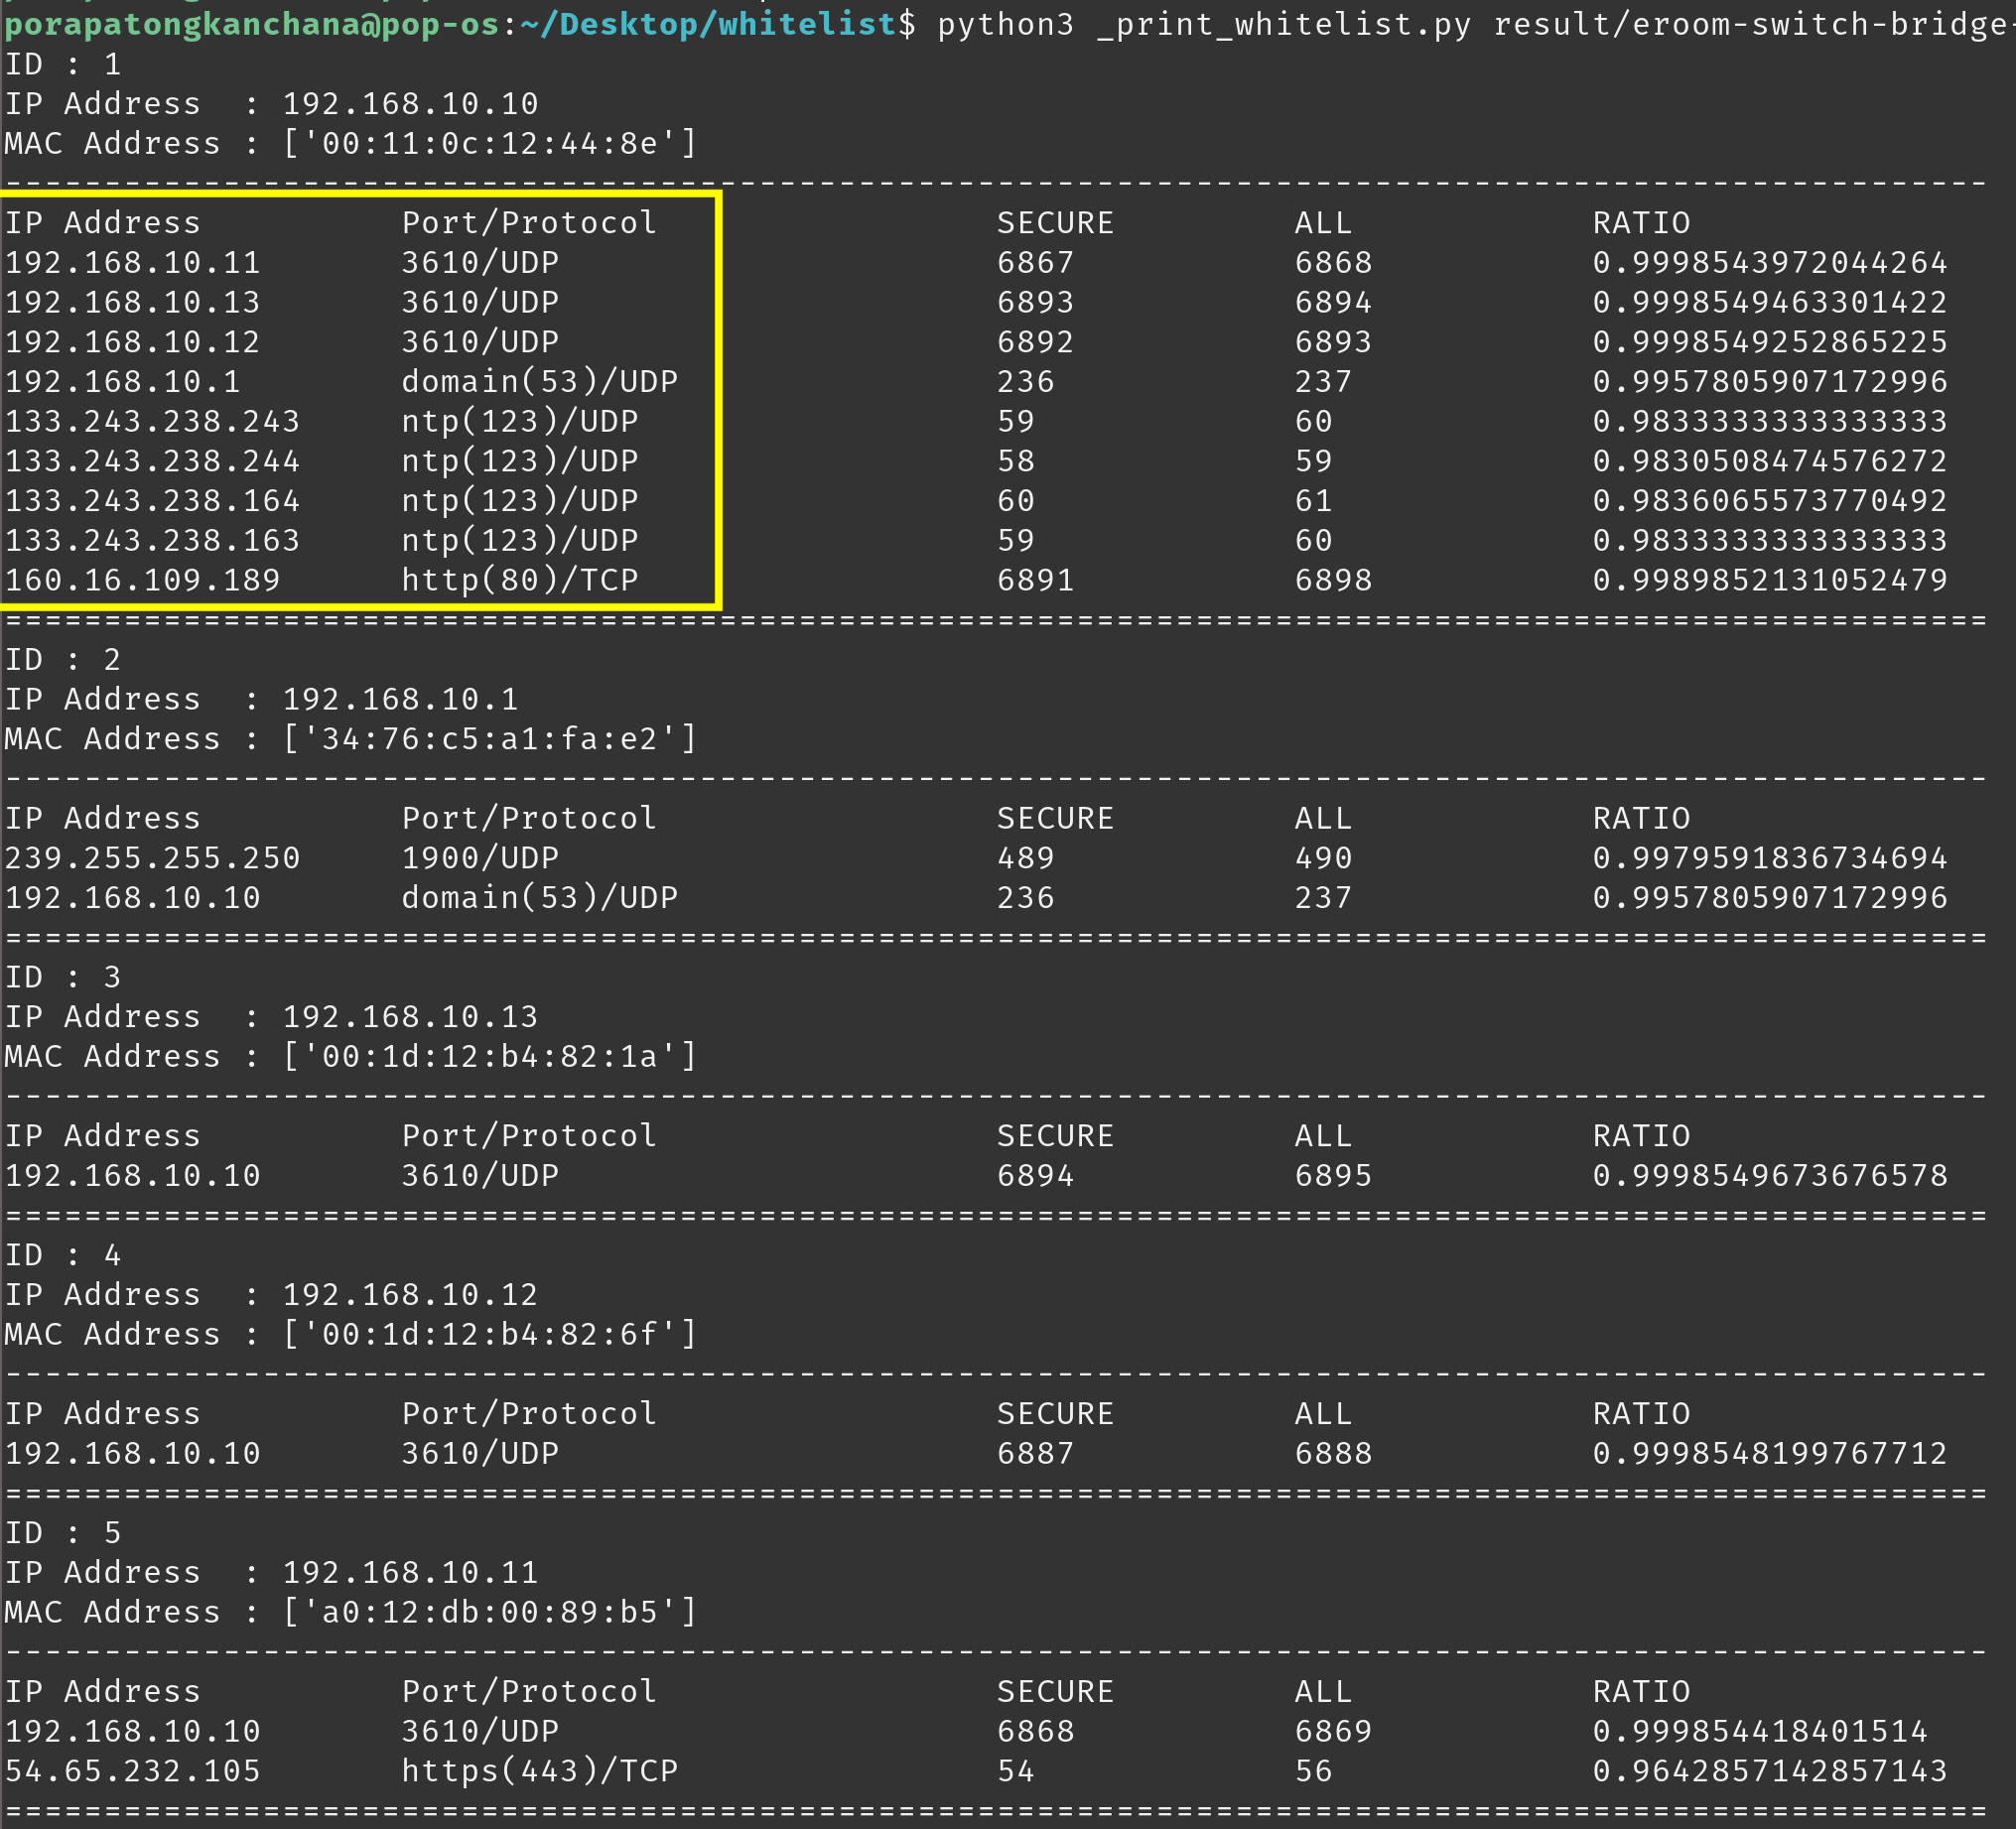
\includegraphics[width=\textwidth]{4_wl_result_eroom}
    \caption{Screenshot of Whitelist Extraction Program (eroom)}
    \label{fig:s4_wl_result_eroom}
\end{figure}

The screenshot of program's output is shown in figure \ref{fig:s4_wl_result_eroom}
The list contained the IP address of hosts, the protocol and port number which our devices started the connection to.
"SECURE" column show the number of time subgroup was judged as secure (First packet was from device).
"ALL" column show number of subgroup packet of this host was found. 

We compared our program's output with our previous inspect in section \ref{packet_capture} and found that
hosts extracted with this algorithm were indeed the secured hosts, proving that the program is working.

\subsection{Discussion} 

The result shows that the algorithm can perform well with our tested IoT devices, taking the advantage of device's limited communication pattern. However, this didn’t mean that this approach would work well on all IoT system, each IoT system has its own protocol, network topology and communication pattern.  

In our tested IoT system, air conditioner controllers take command from the control panel. In this case the control panel is the one initiates the connection to air conditioner controller; therefore, air conditioner should not consider control panel as the secure host and would not add it to the whitelist. However, our tested IoT system is designed so that both control panel and controller are in the same LAN, so we were able to extract both IP addresses. In the case that, control panel locates outside the LAN, we don’t think that this algorithm would work. 

Another worth mentioned topic is that we have conducted this experiment under the assumption that during Preparation stage, no malicious host has already intruded in and all our captured packet is secure. If there were malware in the captured traffic, there is a possibility that our algorithm would recognize it as a secure host and couldn’t create a proper whitelist.   

For the whitelist extraction algorithm improvements, in this current version, we only investigated IPv4 packets, while left the IPv6 untouched. We didn’t consider hosts’ P2P connection, which might happen outside of the switch. 